\subsection{Process variables}\label{chapter_VARIABLES}
This chapter gives a short overview over the controlled process variables, the actuating variables and the set points. The grafic below shows, where these values are placed in the closed loop. \\
The first rectangle represents the controller, that is designed and implemented in this project. The second rectangle represents the quadrocopter; the process that has to be controlled.
\begin{figure}[H]
	\centering
		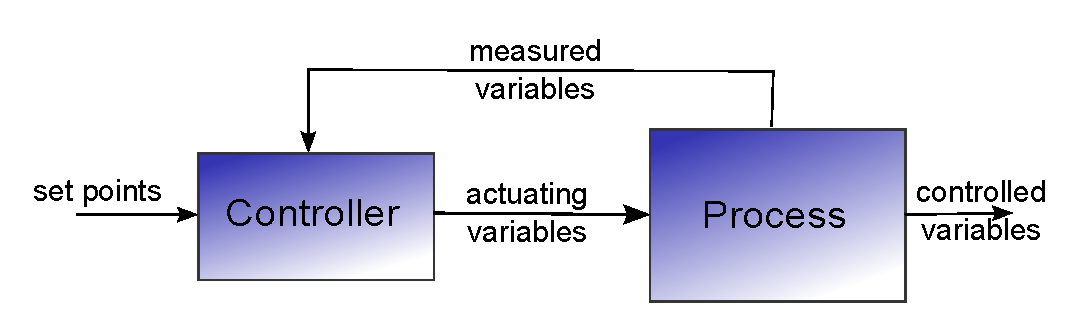
\includegraphics[width=0.9\textwidth]{03_Grafiken/closed_loop_abstract.pdf}
	\caption{closed loop abstract}
	\label{fig:closed loop abstract}
\end{figure}
The set points are equal to the controlled variables. The pilot is able to control the \textit{angle of phi} (roll), the \textit{angle of theta} (pitch) and the \textit{rate of psi} (yaw). In chapter \ref{chapter_BASICS}, one degree of freedom is \textit{thrust}, which in some way also is a set point, but it is not a controlled variable, but directly controlled by the pilot. Actually it is an offset, that is added to the actuating variables, that have been calculated by the controller before.
These actuating variables are some sort of normalized forces, every propeller has to provide. They are called 'pseudo forces' in this document. \\
Last but not least, there are the measured variables, that are needed by the controller. These variables are content of the next chapter.